\chapter{Réseau de neurones \\(Thibault \& Quentin)}

\section{Architecture}

Le réseau de neurones est l'élément au cœur du logiciel d'OCR, il était donc
primordial d'avoir l'implémentation de ce dernier prête dès la première
soutenance. Il fallait un réseau assez flexible afin de permettre
l'apprentissage de reconnaissance de caractères d'ici la prochaine soutenance,
ce qui représentera une tâche majeure. Nous sommes partis sur une architecture
totalement modulaire du réseau, pour faciliter les tests et de ne pas se
retrouver bloqué avec des défauts de conception initiaux tout au long du projet.
L'aspect technique a été découpé en plusieurs parties :

\begin{itemize}
    \item Réflexion théorique de l'implémentation et des besoins.
    \item Implémentation des structures fondamentales : matrices, couches,
        réseau.
    \item Implémentation des fonctions principales du réseau : propagation,
        apprentissage.
\end{itemize}

Chaque étape de développement a necessité des tests avant de passer à l'étape
suivante, afin de s'assurer au maximum de la stabilité des fondements de notre
réseau.

\newpage

Notre réseau de neurones se compose des trois structures suivantes :

\begin{myminted}{neural\_network.h}
struct Layer
{
    size_t nb_neurons;
    struct Matrix *in;
    struct Matrix *out;
    struct Matrix *weight;
    struct Matrix *bias;
    struct Matrix *delta;
};

struct Network
{
    size_t nb_layers;
    struct Layer *layers;
};
\end{myminted}

\begin{myminted}{matrix.h}
struct Matrix
{
    size_t nb_rows;
    size_t nb_cols;
    float *mat;
};
\end{myminted}

L'abstraction à l'aide de matrice aide grandement l'implémentation du réseau,
où chaque formule se résume simplement par des opérations matricielles basiques.
Toutes les fonctions majeures du réseau tiennent en une cinquantaine de lignes
(une grande partie est due à la gestion de la mémoire).

La création d'un réseau de neurones avec cette structure nécessite uniquement de
préciser le nombre de couches, ainsi que leurs tailles respectives. Par exemple
pour notre réseau apprenant la fonction XOR le code est :

\begin{myminted}{xor\_network.c}
size_t layers_size[] = {2, 2, 1};
struct Network *network = network_alloc(3, layers_size);
...
network_free(network);
\end{myminted}

Ceci nous crée le réseau de neurones suivant :

% http://www.texample.net/tikz/examples/neural-network/
\def\layersep{2.5cm}
\vspace{1cm}
\begin{center}
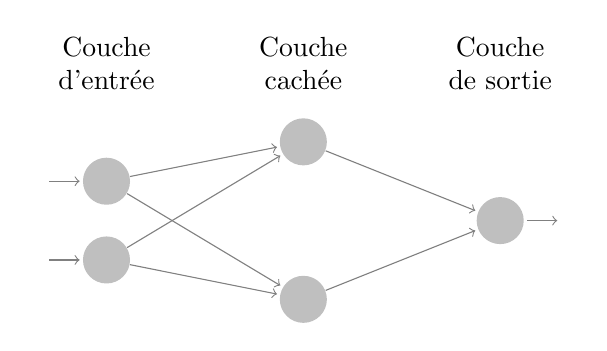
\begin{tikzpicture}[shorten >=1pt,->,draw=black!50, node distance=\layersep]
    \tikzstyle{every pin edge}=[<-,shorten <=1pt]
    \tikzstyle{neuron}=[circle,fill=black!25,minimum size=17pt,inner sep=0pt]
    \tikzstyle{annot}=[text width=4em, text centered]

    % Draw the input layer nodes
    \node[neuron, pin=left:] (I-1) at (0,-1.5) {};
    \node[neuron, pin=left:] (I-2) at (0,-2.5) {};

    % Draw the hidden layer nodes
    \node[neuron] (H-1) at (2.5, -1) {};
    \node[neuron] (H-2) at (2.5, -3) {};

    % Draw the output layer node
    \node[neuron,pin={[pin edge={->}]right:}] (O) at (5, -2) {};

    % Connect every node in the input layer with every node in the
    % hidden layer.
    \foreach \source in {1,...,2}
        \foreach \dest in {1,...,2}
            \path (I-\source) edge (H-\dest);

    % Connect every node in the hidden layer with the output layer
    \foreach \source in {1,...,2}
        \path (H-\source) edge (O);

    % Annotate the layers
    \node[annot,above of=H-1, node distance=1cm] (hl) {Couche cachée};
    \node[annot,left of=hl] {Couche d'entrée};
    \node[annot,right of=hl] {Couche de sortie};
\end{tikzpicture}
\end{center}

\section{Propagation}

Les propagations avant et arrière suivent les principes classiques d'un réseau
de neurones. Les formules utilisées sont sous formes matricielles où $l$ est une
couche quelconque du réseau et $L$ la dernière couche :

\textbf{Propagation avant}

$in^l = weight^l \cdot out^{l-1} + bias^l$

$out^l = \sigma (in^l)$

\newpage

\textbf{Calcul d'erreur}

$delta^L = (out^L − y) \odot \sigma '(in^L)$

Pour un exemple lors de l'apprentissage, $y$ représente la sortie attendue par
le réseau.

\textbf{Rétropropagation}

$delta^l = ((weight^{l+1})^T \cdot delta^{l+1}) \odot \sigma '(in^l)$

\section{Apprentissage}

Pour l'apprentissage du réseau de neurones, l'\textbf{algorithme du gradient} a
été appliqué. Dans l'idée de rester sur une architecture modulaire, il fallait
généraliser le format des exemples donnés pour entraîner le réseau, afin que ce
dernier puisse aussi bien apprendre à partir de résultats d'un XOR que des
pixels d'une image. Pour cela, nous avons utilisé à nouveau notre abstraction de
matrice pour construire les deux structures suivantes :

\begin{myminted}{training.h}
struct TrainingData
{
    struct Matrix *in;
    struct Matrix *out;
};

struct TrainingSet
{
    size_t nb_examples;
    struct TrainingData *examples;
};
\end{myminted}

\newpage

Les formules de l'algorithme de gradient pour mettre à jour les poids et les
bias sont :

$weight^l = weight^l - \frac{\eta}{m} \displaystyle\sum^m{delta^l \cdot (out^{l-1})^T}$

$bias^l = bias^l - \frac{\eta}{m} \displaystyle\sum^m{delta^l}$

Où $\eta$ est le cœfficient d'apprentissage, et $m$ la taille du jeu de données.
Pour la première soutenance, appliquer des sommations sur les $m$ exemples n'est
pas gênant puisque la fonction XOR est constituée uniquement de 4 exemples
(correspondant à la table de vérité). En revanche, pour nos futures images,
découper notre ensemble de données va être nécessaire si l'on veut un
apprentissage bien plus efficace : c'est la méthode du \textit{mini-batch
gradient descent}.

\section{Jeu d'images}

Plusieurs jeux d'images sont déjà disponibles sur Internet, mais la plupart sont
utilisés pour des recherches avancées en traitement d'image et contiennent bien
plus d'informations que nécessaires pour notre utilisation. Nous avons décidé de
générer nos propres données ce qui nous donne un réel contrôle sur ces
dernières. Pour cela, un script Bash prenant une liste de caractères va générer
toutes les images dans différentes polices d'écriture, sous un format BMP de
taille 32x32.

\begin{figure}[H]
    \centering
    \fbox{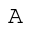
\includegraphics[width=0.2\textwidth]{train_set00}}
    \fbox{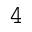
\includegraphics[width=0.2\textwidth]{train_set01}}
    \fbox{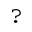
\includegraphics[width=0.2\textwidth]{train_set02}}
    \caption{Extrait du jeu d'images}
\end{figure}

\newpage

\section{Sauvegarde et chargement}

Pour conserver les propriétés du réseau, il est possible de sauvegarder les
poids et biais de chaque couche dans un fichier. De même, l'opération inverse a
été implémentée c'est-à-dire pouvoir charger un réseau depuis un fichier externe
et l'utiliser pour faire tourner les algorithmes.

Le format pour stocker ces informations est simplement un fichier texte de la
forme :

\begin{minted}{text}
    nb_couches
    taille_couche1 taille_couche2 ...
    matrice_poids_couche1
    matrice_biais_couche1
    ...
\end{minted}
